\newpage
\chapter{Имплементација и рендерирање}
\section{Технологии}
Симулаторот е напишан во C++, стандардниот избор во пишување на физички симулатори заради брзината и развиениот екосистем на библиотеки за компјутерска графика. Библиотеките што се користат се:
\begin{itemize}
	\item \textbf{OpenGL 4.3} за рендерирање, избран заради едноставноста и можноста да се додадат compute shaders во иднина
	\item \textbf{GLFW} за креирање прозорец, контекст на OpenGL и читање на влезни настани. Работи на повеќе платформи и е модерен
	\item \textbf{GLAD} за вчитување на OpenGL функциите
	\item \textbf{GLM} за линеарна алгебра (операции со матрици и вектори), лесна интеграција со GLSL векторските типови: glm::vec3, glm::mat4, glm::cross итн.
	\item \textbf{Assimp} за вчитување на мрежите. Конфигуриран само за вчитување на OBJ, FBX, GLTF датотеки за намалување на големина
	\item \textbf{TetGen} за тетраедрализацијата на мрежите
	\item \textbf{ImGui} за приказ на едноставен кориснички интерфејс
\end{itemize}

Овие технологии беа избрани бидејќи овозможуваат лесно извршување на апликацијата на различни платформи со минимална конфигурација.  


\section{Структура на модули}

Апликацијата е поделена на 4 модули кои имаат своја улога.

\textbf{Физика}, јадрото на симулаторот. Нема знаење за OpenGL и приказот на екран. Добива објекти и почетна состојба на влез (меки тела и колајдери), изложува функција за ажурирање на состојбата на објектите во одреден временски интервал и изложува функција за добивање на моменталната положба на сите објекти за да се прикажат од рендерерот. Дополнително се изложуваат методи кои се повикуваат од корисничкиот интерфејс.

\textbf{Рендерирање}, содржи структури за додавање објекти во OpenGL сцената. \textbf{Mesh} класата ги содржи VAO/VBO/EBO и \textbf{draw()} за исцртување на објектите. Содржи и метод \textbf{updateMesh} за ажурирање на позициите на темињата на објектот што се добива од решавачот од модулот за физика.

\textbf{Кориснички интерфејс}, содржи ImGui код за приказ на контролите врз симулаторот. Поврзан е со \textbf{Solver} за промена на состојбата на симулацијата.

\textbf{Поврзување} (\textbf{main.cpp, camera.cpp, shader.cpp, util.hpp} ги поврзуваат трите останати делови.

\section{Процесен тек на апликацијата}
Процесот започнува со вчитување на објектите кои треба да се прикажат во сцената со користење на библиотеката Assimp. Најважното предпроцесирање што го прави Assimp е триангулацијата  на мрежата бидејќи рендерерот претпоставува топологија од триаголници. Од податоците добиени од Assimp моментално само се користат позициите на темињата и страните кои ги индексираат темињата, сите останати податоци се вчитуваат но се игнорираат (UV координати, текстури, материјали итн.). 

По вчитувањето на позициите и индексите иницијализираат баферите потребни за OpenGL да ги  прикаже објектите на екран. Потоа се иницијализираат меките и колизиски тела кои ќе бидат дел од пресметките на решавачот, по што може да почне процесниот тек на рендерирање (rendering loop).

\subsection{Процесен тек на рендерирање}
Најпрво се пресметува изминатото време од претходната слика до моменталната слика. Ова е неопходно за задржувањето на фиксниот временски чекор на решавачот (16.67 ms).  Потоа се процесира кориснички влез кој се користи за движење на камерата околу сцената, по што се ажурира корисничкиот интерфејс и се читаат промените што корисникот ги има направено. 

Доколку  имаат изминато барем 16.67 милисекунди од последното ажурирање на решавачот, повторно се повикува \textbf{update} методот. Овој избор е направен за да се одвои зависноста на физичкото ажурирање од брзината на прикажување на сликите од рендерерот. 

Независно од ажурирањето, се продолжува со припрема за прикажување на сцената на екран. Прво се иницијализира бојата на позадината на сцената, па се припремаат шејдерите и трансформациските матрици кои им се праќаат за точно исцртување на сцената. Најпрво се припрема за исцртување мекото тело, се ажурираат позициите (\textbf{updateMesh}) на честичките и се испраќа на исцртување.  Потоа се припремаат колизиските тела со подесување на нивните трансформациски матрици и се исцртуваат, а на крај се исцртува рамнината што го означува подот.

Врз сцената се исцртува корисничкиот интерфејс, по што се праќа целата слика за приказ на ектран \textbf{glfwSwapBuffers} и за крај се чита корисничкиот влез кој се користи на почетокот на процесниот тек на рендерирање. \ref{fig:rendering-pipeline}

 \begin{figure}[p]
	\centering
	\resizebox{!}{0.92\textheight}{
		\begin{tikzpicture}[
			font=\small,
			node distance=6mm and 10mm,
			box/.style={
				draw, rounded corners=2pt, align=center,
				inner sep=4pt, minimum height=8mm, text width=60mm},
			dec/.style={
				draw, diamond, aspect=2, align=center,
				inner sep=1pt, text width=24mm},
			flow/.style={-{Stealth[length=2mm]}, thick},
			grp/.style={draw, dashed, rounded corners=4pt, inner sep=6mm},
			grplabel/.style={font=\small\itshape, anchor=north west}]
			
			% ---- one-time setup ----
			\node[box] (load)  {\texttt{Model::loadModel}\\Assimp \texttt{ReadFile}\\(Triangulate, FlipUVs)};
			\node[box, below=of load] (proc) {\texttt{processNode / processMesh}\\build Vertex + index arrays};
			\node[box, below=of proc] (init) {\texttt{Mesh::initMesh}\\VAO/VBO/EBO\\interleaved attribs 0,1,2};
			
			\draw[flow] (load) -- (proc);
			\draw[flow] (proc) -- (init);
			
			% ---- per-frame loop: input + update ----
			\node[box, below=14mm of init] (time)  {1.\ Time bookkeeping (deltaTime)};
			\node[box, below=of time]      (input) {2.\ \texttt{processInput} (camera, hotkeys)};
			\node[box, below=of input]     (gui)   {3.\ \texttt{gui.update} };
			
			\draw[flow] (init) -- node[right]{first frame} (time);sher, and shared facilities such as a toilet and a
			\draw[flow] (time)  -- (input);
			\draw[flow] (input) -- (gui);
			
			% ---- fixed-timestep accumulator (now before rendering) ----
			\node[dec, below=10mm of gui] (acc) {accumulator $\ge$ dt?};
			\node[box, below=8mm of acc]  (upd) {\texttt{solver.update(dt)}\\(substep loop inside, \S4.5)};
			\node[box, below=of upd]      (dec) {\texttt{accumulator -= dt}};
			
			\draw[flow] (gui)  -- (acc);
			\draw[flow] (acc)  -- node[right]{yes} (upd);
			\draw[flow] (upd)  -- (dec);
			\draw[flow] (dec.east) -- ++(36mm,0) |- (acc.east);
			
			% ---- render ----
			\node[box, below=10mm of dec] (clear) {5.\ Clear color + depth buffers};
			\node[box, below=of clear]    (unif)  {6.\ Set shader uniforms\\(model/view/projection, light)};
			\node[box, below=of unif]     (getpos){7.\ \texttt{getParticlePositions()}\\first $N$ surface
				particles};
			\node[box, below=of getpos]   (upmesh) {\texttt{Mesh::updateMesh}\\mutate vertices +
				\texttt{glBufferSubData}};
			\node[box, below=of upmesh]   (drawsb) {\texttt{cubeModel.Draw} (soft body)};
			\node[box, below=of drawsb]   (drawc)  {8.\ Draw colliders and ground plane};
			\node[box, below=of drawc]    (drawgui){9.\ \texttt{gui.draw} (overlay)};
			\node[box, below=of drawgui]  (swap)   {10.\ \texttt{glfwSwapBuffers} + \texttt{pollEvents}};
			
			\draw[flow] (acc.west) -- node[above,sloped]{no} ++(-30mm,0) |- (clear.west);
			\draw[flow] (clear)   -- (unif);
			\draw[flow] (unif)    -- (getpos);
			\draw[flow] (getpos)  -- (upmesh);
			\draw[flow] (upmesh)  -- (drawsb);
			\draw[flow] (drawsb)  -- (drawc);
			\draw[flow] (drawc)   -- (drawgui);
			\draw[flow] (drawgui) -- (swap);
			
			% next-frame back-edge
			\draw[flow] (swap.east) -- ++(46mm,0) |- node[above,pos=0.25,sloped]{next frame} (time.east);
			
			% ---- grouping boxes (drawn behind) ----
			\begin{scope}[on background layer]
				\node[grp, fit=(load)(init)] (setupbox) {};
				\node[grplabel] at (setupbox.north west) {One-time setup};
				
				\node[grp, fit=(acc)(dec)] (accbox) {};
				\node[grplabel] at (accbox.north west) {4.\ Fixed-timestep accumulator};
			\end{scope}
			
		\end{tikzpicture}
	}
	\caption[Rendering pipeline and per-frame loop]{%
		The rendering pipeline. One-time asset setup (top) feeds the GPU buffers
		once. The per-frame loop handles input, then advances physics via a
		fixed-timestep accumulator, and only afterwards clears the buffers and
		re-uploads the surface particles for drawing. Step numbers correspond to
		the annotated frame loop in \texttt{main.cpp}.}
	\label{fig:rendering-pipeline}
\end{figure}

\subsection{Ажурирање на површината на мекото тело}
Чекорот од процесниот тек на рендерирање што е најрелевантен за перформансите е ажурирањето на мрежата на мекото тело во \textbf{updateMesh}. На влез се добиваат новите позиции на честичките од мекото тело и се прави ажурирање на баферот кој се наоѓа на графичкиот процесор.  Дополнително, кога се земаат најновите позиции на честичките од \textbf{getParticlePositons} се добиваат само честичките што се наоѓаат на површината на мекото тело, односно оригиналните влезни темиња добиени од Assimp.  Моментално начинот на кој се добиваат оригиналните честички е со земање на првите \textbf{numSurfaceParticles} елементи од низата на позиции на честичките. Поради инваријантноста на индекси добиени од 4.2 (TetGen), тие влезови соодветсвуваат со оригиналните влезни темиња во првичниот редослед. Внатрешните точки генерирани од TetGen никогаш не се прикажуваат.

Претпоставката дека првите \textbf{numSurfaceParticles} соодветствуваат со оригиналните темиња зависи од знамето \textit{Y} на TetGen. Побезбеден пристап би бил да се направи мапирање помеѓу индексите во решавачот и индексите кои се праќаат на рендерирање.

\subsection{Шејдери (shaders)}
За рендерирање се користи само еден пар на вертекс/фрагмент шејдери (vertex/fragment). \textbf{particle.vert/particle/frag} се користат за сенчање на мекото тело, колизиските објекти и земјата. Се користи Phong осветлување со едно точкесто светло. Моментално материјалот на објектот е само бојат која се менува преку униформна променлива, исто како и бојата на светлото. Model, view, projection матриците се извлекуваат од објектот на камерата.

\section{Контроли на апликацијата}
\subsection{Кориснички интерфејс}
Како што беше спомнато во воведот, корисничкиот интерфејс е креиран со помош на библиотеката ImGui. Тој е едноставен панел кој овозможува контрола на одредени параметри на симулацијата:
\begin{itemize}
	\item \textbf{Избирање на објект за меко тело}. Овозможува на корисникот да го избере мекото тело за кое сака да се изврши симулацијата
	\item \textbf{Копче за ресетирање}. При притискање на копчето од интерфејсот или притискање 'R' на тастатурата, се враќа симулацијата во првобитната состојба
	\item \textbf{Лизгач(slider) за подесување на попустливост}. Дозволува промена на параметарот $\alpha$ за попустливост, но log10 со ранг од $10^{-10}$(скоро цврсто тело) до $10^0=1.0$(многу попустливо).
	\item \textbf{Лизгач за број на итерации на решавачот}
	\item \textbf{Лизгачи за промена на позиција и големина на колизиски тела}
	\item \textbf{Бројач за слики во секунда (frames per second)}
\end{itemize}

\begin{figure}[h]
	\centering
	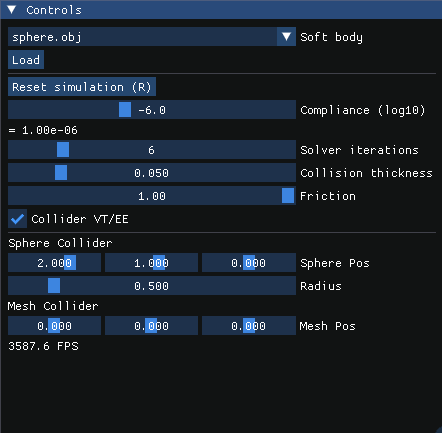
\includegraphics[width=0.8\linewidth]{template/ui.png}
	\caption{Слика од корисничкиот интерфејс}
	\label{fig:ui}
\end{figure}

\subsection{Контроли на тастатура и камера}
Овие контроли се однесуваат на движењето низ сцената

\begin{table}[h]
	\centering
	\begin{tabular}{@{}cl@{}}
		\toprule
		\textbf{Копче} & \textbf{Акција} \\
		\midrule
		\texttt{RMB}          & Вклучи менување на аголот на камерата (при држење) \\
		\texttt{WASD}         & Хоризонтално движење на камерата. (во однос на коорд. систем на камерата) \\
		\texttt{EQ}           & Вертикално движење на камерата. (во однос на коорд. систем на камерата)\\
		\texttt{G} / \texttt{F} & Вклучување на wireframe режим / вклучување на режим со пополнети триаголници\\
		\texttt{R}            & Ресетирање на симулацијата. \\
		\texttt{Escape}       & Излез. \\
		\bottomrule
	\end{tabular}
	\caption{Тастатурни кратенки}
	\label{tab:controls}
\end{table}

\subsection{Забелешка за перформанси}

Симулаторот работи целосно на една нишка од процесорот. Секој дел од ажурирањето на решавачот: предвидување позиции, решавање ограничувања, колизии, е секвенцијално. Ова нормално ги ограничува перформансите до тоа што може да постигне едно јадро на процесорот. Додавањето на паралелизам не е тривијално и е надвор од опсегот на овој труд.

Дополнително, графичкиот процесор (GPU) се користи само за рендерирање, иако постои можност за предавање на дел од пресметките од симулаторот на GPU, што повторно е надвор од опсегот и можност за идно подобрување. 